\documentclass[portrate,a0paper,fontscale=0.45,margin=1cm]{baposter}
%\documentclass[landscape,paperwidth=1682mm,paperheight=1189mm,fontscale=0.4,margin=3cm]{baposter}

\usepackage{calc}
\usepackage{graphicx}
\usepackage{amsmath}
\usepackage{amssymb}
\usepackage{relsize}
\usepackage{multirow}
\usepackage{rotating}
\usepackage{bm}
\usepackage{enumitem}
\usepackage{booktabs}
\usepackage{relsize}		% For \smaller
\usepackage{url}			% For \url

\usepackage{graphicx}
\usepackage{multicol}
\usepackage{subcaption}
\captionsetup{compatibility=false}

\usepackage{nameref}
%\usepackage{times}
%\usepackage{helvet}
%\usepackage{bookman}
\usepackage{palatino}
%% Pablo's personal packages
%% AMS unofficial LateX proceeding template:
%%    http://www.cimms.ou.edu/~lakshman/ametsoc/
%%\usepackage[hypertex]{hyperref}
%% end personal packages

%\newcommand{\captionfont}{\footnotesize}

\graphicspath{{images/}{./images}}
\usetikzlibrary{calc}


\newcommand{\Matrix}[1]{\begin{bmatrix} #1 \end{bmatrix}}
\newcommand{\Vector}[1]{\begin{pmatrix} #1 \end{pmatrix}}

\newcommand*{\norm}[1]{\mathopen\| #1 \mathclose\|}% use instead of $\|x\|$
\newcommand*{\abs}[1]{\mathopen| #1 \mathclose|}% use instead of $\|x\|$
\newcommand*{\normLR}[1]{\left\| #1 \right\|}% use instead of $\|x\|$

\newcommand*{\SET}[1]  {\ensuremath{\mathcal{#1}}}
\newcommand*{\FUN}[1]  {\ensuremath{\mathcal{#1}}}
\newcommand*{\MAT}[1]  {\ensuremath{\boldsymbol{#1}}}
\newcommand*{\VEC}[1]  {\ensuremath{\boldsymbol{#1}}}
\newcommand*{\CONST}[1]{\ensuremath{\mathit{#1}}}

\DeclareMathOperator*{\argmax}{arg\,max}
\DeclareMathOperator*{\diag}{diag}
\DeclareMathOperator*{\argmin}{arg\,min}
\DeclareMathOperator*{\vectorize}{vec}
\DeclareMathOperator*{\reshape}{reshape}

%\font\dsfnt=dsrom12

\newcommand{\SNN}{\ensuremath{\mathbb N}}
\newcommand{\SRR}{\ensuremath{\mathbb R}}
\newcommand{\SZZ}{\ensuremath{\mathbb Z}}
%-----------------------------------------------------------------------------
% Matrices of the shape model
\renewcommand{\a}{\VEC\alpha}
\renewcommand{\v}{\VEC v}
\renewcommand{\l}{\VEC l}
\newcommand*{\m}{\VEC{\mu}}
\newcommand*{\M}{\MAT{M}}
\renewcommand*{\P}{\MAT{\Pi}}

%\newcommand{\J}{\SET J}
\newcommand{\J}{\SET{P}}
\newcommand{\Active}{\mathcal{A}}
\newcommand{\Selection}{\mathbf{S}}
\newcommand{\AllSelections}{\mathfrak{S}}
\newcommand{\Params}{\VEC\Theta}

%%%%%%%%%%%%%%%%%%%%%%%%%%%%%%%%%%%%%%%%%%%%%%%%%%%%%%%%%%%%%%%%%%%%%%%%%%%%%%%%
%%%% Some math symbols used in the text
%%%%%%%%%%%%%%%%%%%%%%%%%%%%%%%%%%%%%%%%%%%%%%%%%%%%%%%%%%%%%%%%%%%%%%%%%%%%%%%%

%%%%%%%%%%%%%%%%%%%%%%%%%%%%%%%%%%%%%%%%%%%%%%%%%%%%%%%%%%%%%%%%%%%%%%%%%%%%%%%%
% Multicol Settings
%%%%%%%%%%%%%%%%%%%%%%%%%%%%%%%%%%%%%%%%%%%%%%%%%%%%%%%%%%%%%%%%%%%%%%%%%%%%%%%%
\setlength{\columnsep}{1.5em}
\setlength{\columnseprule}{0mm}

%%%%%%%%%%%%%%%%%%%%%%%%%%%%%%%%%%%%%%%%%%%%%%%%%%%%%%%%%%%%%%%%%%%%%%%%%%%%%%%%
% Save space in lists. Use this after the opening of the list
%%%%%%%%%%%%%%%%%%%%%%%%%%%%%%%%%%%%%%%%%%%%%%%%%%%%%%%%%%%%%%%%%%%%%%%%%%%%%%%%
\newcommand{\compresslist}{%
\setlength{\itemsep}{1pt}%
\setlength{\parskip}{0pt}%
\setlength{\parsep}{0pt}%
}

%%%%%%%%%%%%%%%%%%%%%%%%%%%%%%%%%%%%%%%%%%%%%%%%%%%%%%%%%%%%%%%%%%%%%%%%%%%%%%
%%% Begin of Document
%%%%%%%%%%%%%%%%%%%%%%%%%%%%%%%%%%%%%%%%%%%%%%%%%%%%%%%%%%%%%%%%%%%%%%%%%%%%%%

\begin{document}

%%%%%%%%%%%%%%%%%%%%%%%%%%%%%%%%%%%%%%%%%%%%%%%%%%%%%%%%%%%%%%%%%%%%%%%%%%%%%%
%%% Here starts the poster
%%%---------------------------------------------------------------------------
%%% Format it to your taste with the options
%%%%%%%%%%%%%%%%%%%%%%%%%%%%%%%%%%%%%%%%%%%%%%%%%%%%%%%%%%%%%%%%%%%%%%%%%%%%%%
% Define some colors

\definecolor{silver}{cmyk}{0,0,0,0.3}
\definecolor{yellow}{cmyk}{0,0,0.9,0.0}
\definecolor{reddishyellow}{cmyk}{0,0.22,1.0,0.0}
\definecolor{black}{cmyk}{0,0,0.0,1.0}
\definecolor{white}{rgb}{1,1,1}
\definecolor{red}{rgb}{.9,0,0}
\definecolor{green}{rgb}{0,.3,0}
\definecolor{blue}{rgb}{.21,.24,.36}

\definecolor{darkYellow}{cmyk}{0,0,1.0,0.5}
\definecolor{darkSilver}{cmyk}{0,0,0,0.1}

\definecolor{middlegray}{rgb}{.4,.4,.4}
\definecolor{lightgray}{rgb}{.7,.7,.7}

\definecolor{lightgreen}{rgb}{.7,7,.35}
\definecolor{lightlila}{rgb}{.6,.6,.8}
\definecolor{lightorange}{rgb}{.88,.74,.15}
\definecolor{lighterorange}{rgb}{.98,.84,.45}
\definecolor{middleblue}{rgb}{.447,.537,.9513}
\definecolor{lightblue}{rgb}{.447,.537,.6313}
\definecolor{lighterblue}{rgb}{.568,.639,.709}
\definecolor{lighteryellow}{cmyk}{0,0,0.1,0.0}
\definecolor{lightestblue}{rgb}{.6,.7,.8}

%%% Setting Background Image %%%%%%%%%%%%%%%%%%%%%%%%%%%%%%%%%%%%%%%%%%%%%%%%%%
\background{
	\begin{tikzpicture}[remember picture,overlay]%
	\draw (current page.north west)+(-0em,0em) node[anchor=north west]
	{
\includegraphics[height=1.01\textheight]{uni_leipzig-bg.jpg}};%{BG_ADMIRARI.jpg}};%
	\end{tikzpicture}
}


%\hyphenation{resolution occlusions}
%%
\begin{poster}%
  % Poster Options
  {
  % Show grid to help with alignment
  grid=false, %true,
  % Number of columns
  columns=3,
  % Column spacing
  colspacing=1.0em,
  % Color style
  bgColorOne= red, %white, %lightgreen, %silver,
  bgColorTwo= white, %white, %middlegray, %lightestblue, %white,
  borderColor=gray, %reddishyellow, %lightorange,
  headerColorOne=darkSilver, %lighterblue, %lightblue,   %lightblue,
  headerColorTwo=lightgray, 
  headerFontColor=black, %lightorange, %black,
  boxColorOne=darkSilver, %darkSilver, %darkblue, %darkYellow,
  boxColorTwo=red, %white,
  % Format of textbox
  textborder=faded,
  % Format of text header
  eyecatcher=true,
  headerborder=none, %open, %none,
  headerheight=0.135\textheight,
  %textfont=\sc, %An example of changing the text font
  headershape=rounded, %smallrounded,
  headershade=shadeLR,
  headerfont=\LARGE\bf,  %%\Large\bf\textsc, %Sans Serif
  textfont={\color{black}\setlength{\parindent}{1.5em}},
  boxshade=none, %shadeTB, %shadeLR,
  background=user, %shadeTB,
  linewidth=2.5pt
  }
  % Eye Catcher
  {
  	\begin{tabular}{l}
      
\includegraphics[height=7.0em]{uni_leipzig-logo.jpg}\\
      \vspace{+3em}
      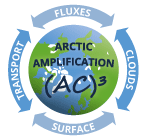
\includegraphics[height=6.0em]{logo_small-ac3.png}
      %\hspace{3em}
      %\includegraphics[height=3.0em]{PosterNumber.png}
      
      %\includegraphics[height=4.0em]{urad2016.png}
    \end{tabular}   
  }
  % Title
  {
  	Studying the Influence of Sea Ice Lead Fraction on Wintertime\\Cloud Macro- and Microphysical Properties During MOSAiC
  }
  % Authors
  {\vspace{+1em} Pablo Saavedra~Garfias$^{1}$, Heike Kalesse-Los$^{1}$, Luisa von~Aldebyll$^{2}$, Hannes Griesche$^{3}$, Gunnar Spreen$^{4}$\\
    $^1$University of Leipzig, Institute for Meteorology, Faculty of Physics and Geosciences\\
    %$^2$University of Cologne, Institute of Geophysics and Meteorology\\
    $^2$Alfred Wegener Institute, Helmholtz Centre for Polar and Marine Research (AWI)\\
    $^3$Leipzig Institute for Tropospheric Research (TROPOS)\\
    $^4$Institute of Environmental Physics, University of Bremen
	%Contact: \url{pablo.saavedra@uni-leipzig.de}
    %% {\color{blue} \url{www2.meteo.uni-bonn.de/admirari}}
   }
  % University logo
  {% The makebox allows the title to flow into the logo, this is a hack
   % because of the L shaped logo.
    %\begin{tabular}{r}
   	%\vspace{+20em}\\
    %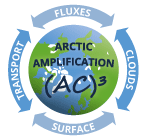
\includegraphics[height=3.0em]{logo_small-ac3.png}
    %\end{tabular}   
  }

%%%%%%%%%%%%%%%%%%%%%%%%%%%%%%%%%%%%%%%%%%%%%%%%%%%%%%%%%%%%%%%%%%%%%%%%%%%%%%
%%% Now define the boxes that make up the poster
%%%---------------------------------------------------------------------------
%%% Each box has a name and can be placed absolutely or relatively.
%%% The only inconvenience is that you can only specify a relative position 
%%% towards an already declared box. So if you have a box attached to the 
%%% bottom, one to the top and a third one which should be in between, you 
%%% have to specify the top and bottom boxes before you specify the middle 
%%% box.
%%%%%%%%%%%%%%%%%%%%%%%%%%%%%%%%%%%%%%%%%%%%%%%%%%%%%%%%%%%%%%%%%%%%%%%%%%%%%%
    %
    % A coloured circle useful as a bullet with an adjustably strong filling
    \newcommand{\colouredcircle}{%
      \vspace{1em}\tikz{\useasboundingbox (-0.2em,-0.32em) rectangle(0.2em,0.32em); \draw[draw=black,fill=lightblue,line width=0.03em] (0,0) circle(0.28em);}\hspace{0.8em}}

% PSG: my ancillary commands:
\newcommand{\polarstern}{RV~\emph{Polarstern}\,}
\newcommand{\mosaic}{\emph{MOSAiC}\,}
\newcommand{\refp}[1]{[\ref{#1}]}
% ----/

%%%%%%%%%%%%%%%%%%%%%%%%%%%%%%%%%%%%%%%%%%%%%%%%%%%%%%%%%%%%%%%%%%%%%%%%%%%%%%
  \headerbox{1.- Research Objectives}{name=objective,column=0,span=1,row=0}{
%%%%%%%%%%%%%%%%%%%%%%%%%%%%%%%%%%%%%%%%%%%%%%%%%%%%%%%%%%%%%%%%%%%%%%%%%%%%%%
The study focuses on the observation of Arctic clouds and sea ice leads to address the following research questions:
\begin{itemize}
	\item Are cloud properties influenced by the presence of sea ice leads?
	\item In which way does the coupling/decoupling of clouds to moisture-layers impact the cloud's properties?
\end{itemize}

\begin{tabular*}{0.99\textwidth}[h!]{lr}
	\begin{minipage}{0.7\textwidth}
		\vspace{-4em}
	{\small Of main interest is the wintertime/early spring legs 1 to 3 of the \mosaic expedition~\refp{bib:Shupe2022} when sea ice leads occured. Instrumention and data set are mainly provided by the Atmospheric Radiation Measurement’s (ARM) Mobile Facility 1 (AMF-1) and by the OCEANET-Atmosphere container from TROPOS.}
	\end{minipage}
	&
	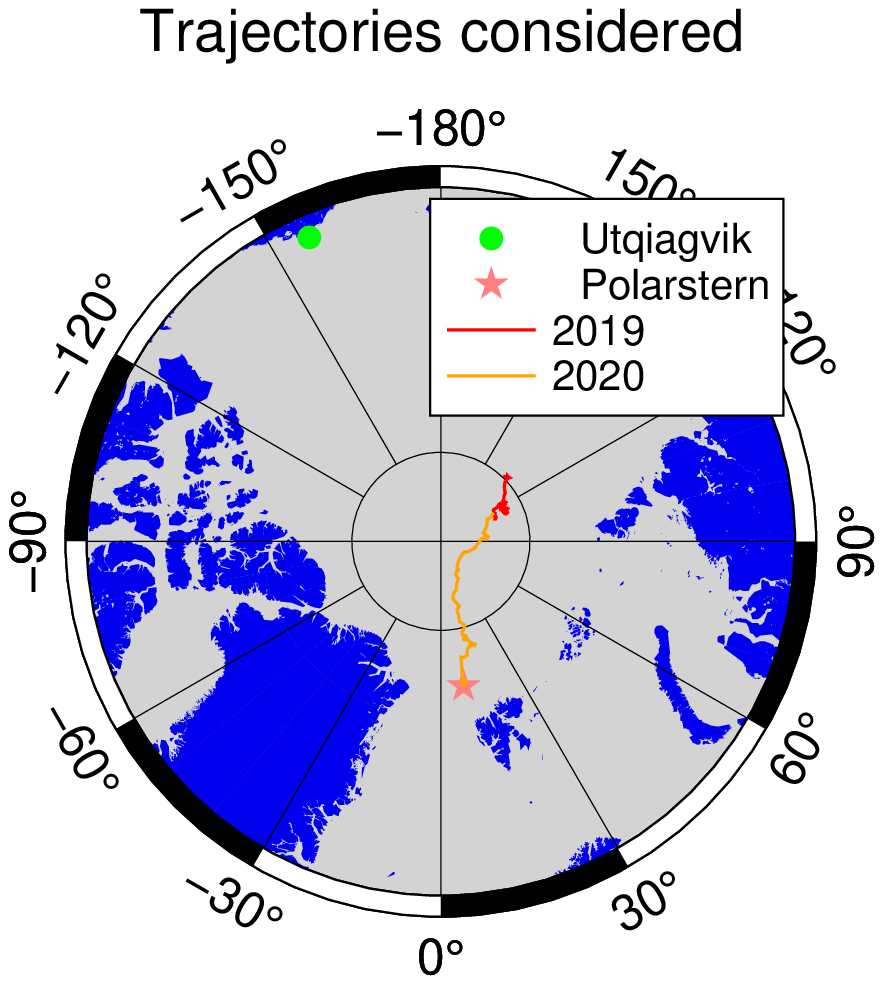
\includegraphics[scale=0.28]{arctic_Pstern_drift20192020.png}	
\end{tabular*}
\\
The case study of 18 Nov 2019 is used to highlight the reseach methods.
  }
%%%%%%%%%%%%%%%%%%%%%%%%%%%%%%%%%%%%%%%%%%%%%%%%%%%%%%%%%%%%%%%%%%%%%%%%%%%%%%
\headerbox{2.- Coupling of Sea Ice and Clouds}{name=methods,column=0,below=objective}{
%%%%%%%%%%%%%%%%%%%%%%%%%%%%%%%%%%%%%%%%%%%%%%%%%%%%%%%%%%%%%%%%%%%%%%%%%%%%%%
%\hspace{-2em}
Daily sea ice lead fraction (LF) is obtained from space-borne observations based on the divergence calculations from consecutive Sentinel-1 SAR scenes~\refp{bib:vonAlbedyll2021}. Additionally, sea ice concentration (SIC) is also provided by the University of Bremen~\refp{bib:Ludwig2021}. Fig.~\ref{fig:lf_sic} summarizes the LF and SIC during the period of interest.
\begin{minipage}{0.99\textwidth}
	%\setcaptiontype{figure}
	\centering
	%\subfloat{
		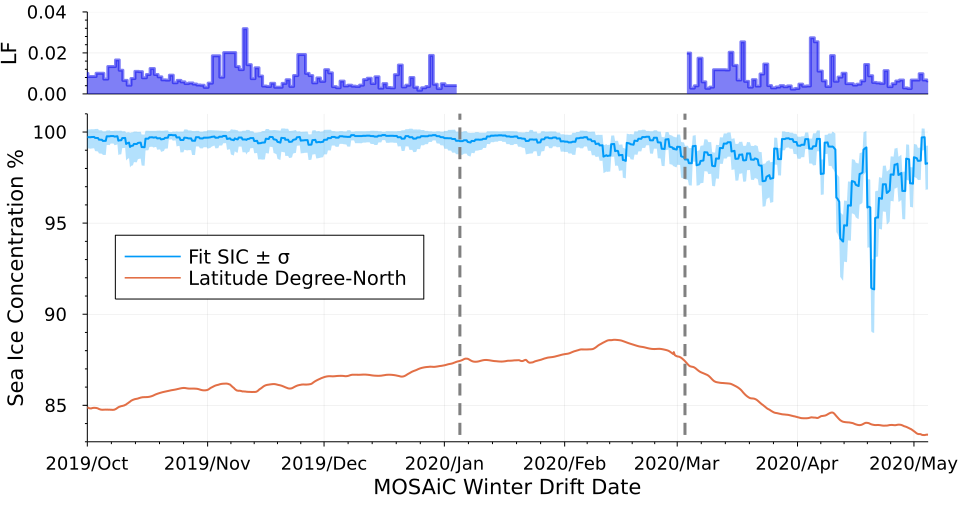
\includegraphics[width=.61\linewidth]{bias_sic_timeseries.png}\hfill
		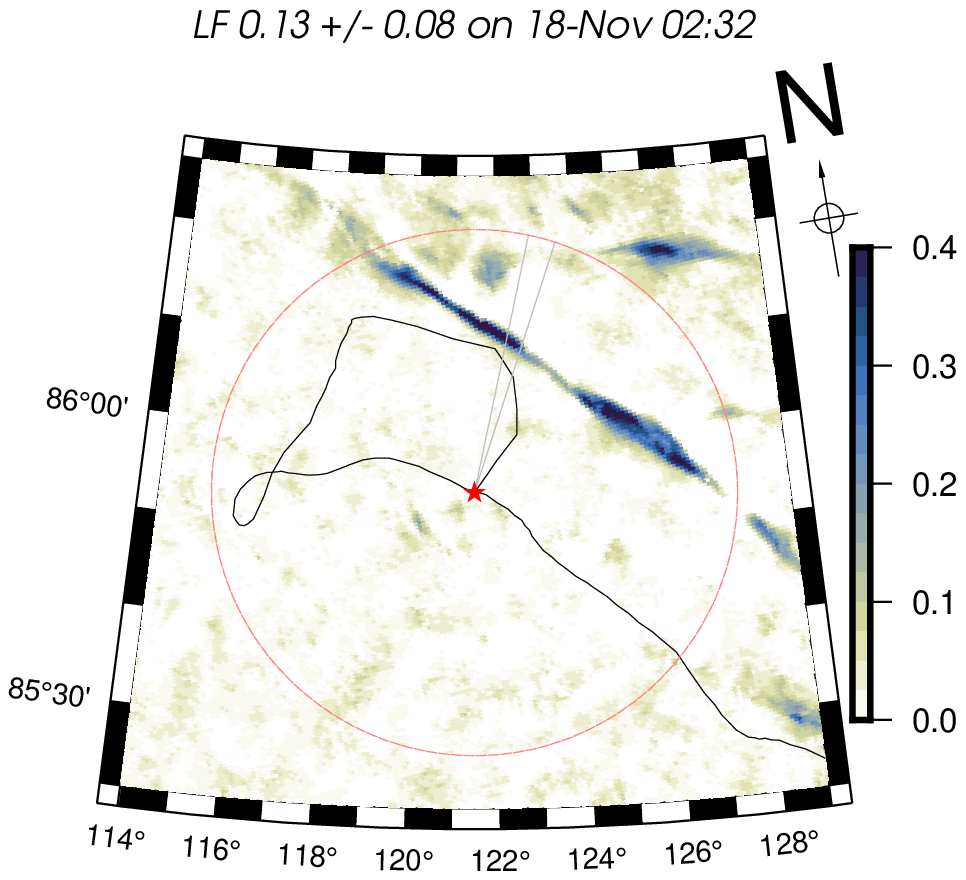
\includegraphics[width=.35\linewidth]{mosaic0152_20191115T03271573_20191118T05301574_LF.png}
	%}
	\captionsetup{width=0.8\linewidth}
	\captionof{figure}{\small Left: LF and SIC for \mosaic leg 1 to 3. Vertical dashed-grey lines indicates period without Sentinel-1 data. Right: case study 18 Nov 2019.}
	\label{fig:lf_sic}
\end{minipage}

The following analysis is performed to relate sea ice lead fraction to cloud observations above \polarstern:

\colouredcircle LF products is analyzed for a sector 50~km around the \polarstern (red star in Fig.~\ref{fig:lf_sic}, right) with updated coordinates every minute.\\

\colouredcircle Sea ice - atmosphere coupling conceptual model\\
Vertical gradient of water vapour transport ($\nabla WVT$) is calculated from specific humidity $q_v~\mathrm{[g~g^{-1}]}$ and horizontal wind $\vec{v}_w~\mathrm{[m~s^{-1}]}$ from radiosonde profiles, following
\begin{equation}
	\nabla \mathrm{WVT} = -\frac{10^2}{g}~|q_v\cdot \vec{v}_w|~\frac{dP}{dz}
\end{equation}
The direction of maximum transport (see grey lines in Fig.~\ref{fig:lf_sic}) is used to relate LF with zenith observations at \polarstern.
\begin{minipage}{0.9\textwidth}
	%\setcaptiontype{figure}
	\centering
	%\subfloat{
		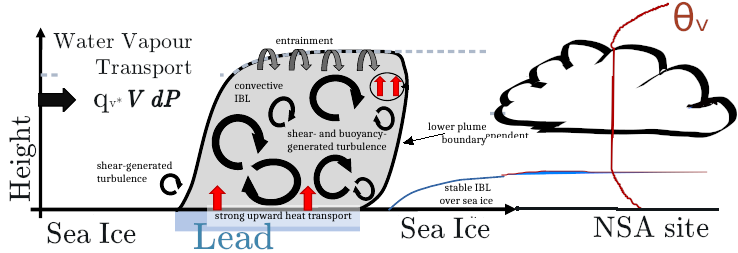
\includegraphics[width=.6\linewidth]{drawing_lead_cloud.png}
	%}
	\captionof{figure}{\smaller Sea ice interaction with observed clouds. Adapted from [\ref{bib:jannos2022}]}
	\label{fig:leadcloud}
\end{minipage}\\

\colouredcircle Planetary boundary layer height (PBLH)\\
The PBLH is used as top layer from which the maximum $\nabla WVT$ is localized downwards. To have a rough estimation of PBLH, the bulk Richardson number defined as
\begin{equation}
	Ri_b(z)\,=\,\frac{g}{\theta_v}\frac{\Delta \theta_v \,\Delta z}{\left( \Delta u \right)^2\,+\,\left(\Delta v \right)^2}
	\label{eq:Rib}
\end{equation}
with $g$ is the constant of gravity 9.81~$\rm m~s^{-2}$, $\theta_v$ is the virtual potential temperature profile
in K, $\Delta \theta_v\,=\,\theta_v-\theta_v(z_0)$, $\Delta u\,=\,u-u_0$, and $\Delta v\,=\,v-v_0$, the horizontal wind components in $\rm m~s^{-1}$. The $\Delta z\,=\,z - z_0$ with $z$ the altitude of the atmosphere layers in $\rm m$ and the subscript $0$ indicating the surface reference.

\colouredcircle Cloud coupling classification: criteria based on the virtual potential temperature $\theta_v$ and location of maximum $\nabla~WVT$ below PBLH. The $\theta_v$ is analyzed to classify cases where the WVT is coupled or decoupled to the cloud.
\begin{minipage}{0.98\linewidth}
	%\setcaptiontype{figure}
	\centering
	%\subfloat{
		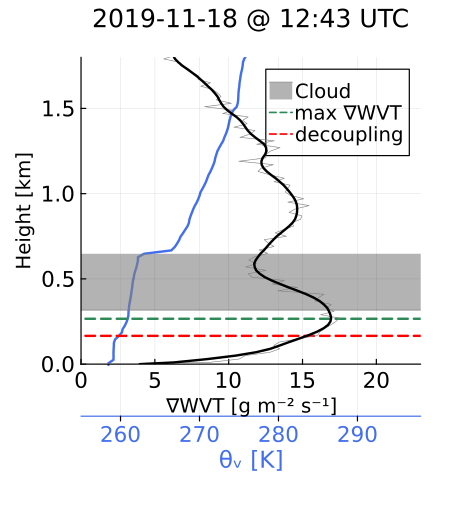
\includegraphics[width=0.32\linewidth]{high_coupling_profile_1243UTC.png}
		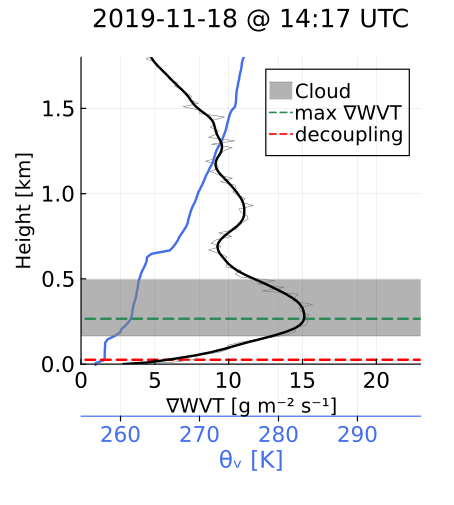
\includegraphics[width=0.32\linewidth]{low_coupling_profile_1417UTC.png}
		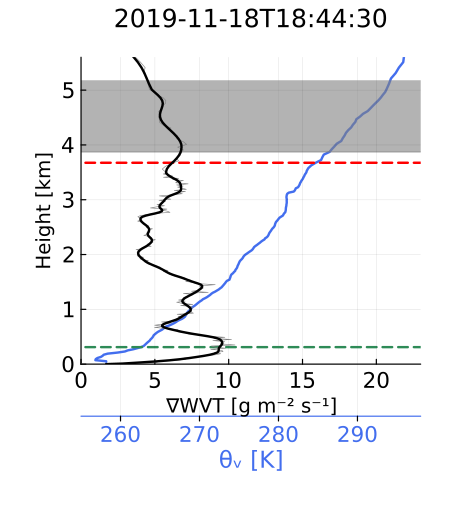
\includegraphics[width=0.32\linewidth]{decoupling_profile_1844UTC.png}
	%}
	\captionof{figure}{\smaller Examples of cloud coupling (left \& middle) and decoupling (right).}
	\label{fig:cop-dec}
\end{minipage}

} % end of box

%%%%%%%%%%%%%%%%%%%%%%%%%%%%%%%%%%%%%%%%%%%%%%%%%%%%%%%%%%%%%%%%%%%%%%%%%%%%%%
  \headerbox{3.- Results for cloud-sea ice coupled case study 18th Nov 2019}{name=results,column=1,row=0,span=2}{
%%%%%%%%%%%%%%%%%%%%%%%%%%%%%%%%%%%%%%%%%%%%%%%%%%%%%%%%%%%%%%%%%%%%%%%%%%%%%%
{\Large Cloudnet target classification is used to determine cloud macro- and microphysical properties. Radiosonde observations are exploited to obtain information on the thermodynamic states of the atmosphere, e.g. $\theta_v$, $\nabla WVT$, wind vectors, and $Ri_b$.}\\
\vspace{+1.5em}
\begin{tabular}{cc} %{@{}lcr@{}}
	\multicolumn{2}{l}{\vspace{+1em}\colouredcircle {\large Synergy of the ship-based zenith observations are needed to apply the Cloudnet classification algorithm.\hfill}} \\
	%\textbf{\Large COUPLED}	& \textbf{\Large DECOUPLED} \\
	\begin{minipage}{0.5\linewidth}
		\begin{center}
			%\setcaptiontype{figure}
			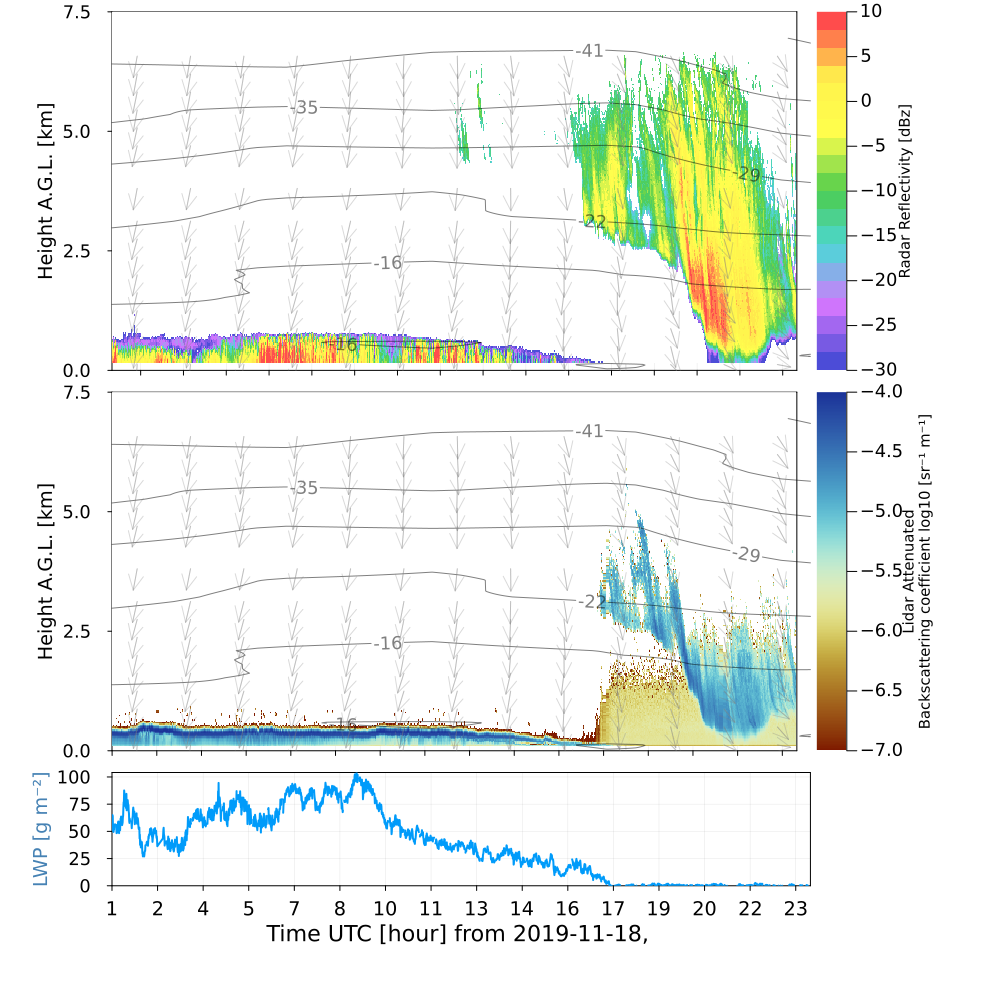
\includegraphics[width=.7\linewidth]{cloudnet_measurements_20191118.png}\\
			\captionsetup{width=0.8\linewidth}
			\captionof{figure}{From top to bottom: ARM KAZR cloud radar reflectivity, ARM ceilometer backscattering coefficient, and liquid water path from HATPRO microwave radiometer~\ref{bib:Ebell2022}.}
			\label{fig:measurements}
		\end{center}
	\end{minipage}
	&
	\begin{minipage}{0.4\linewidth}	
		\begin{center}             
			%\setcaptiontype{figure}
			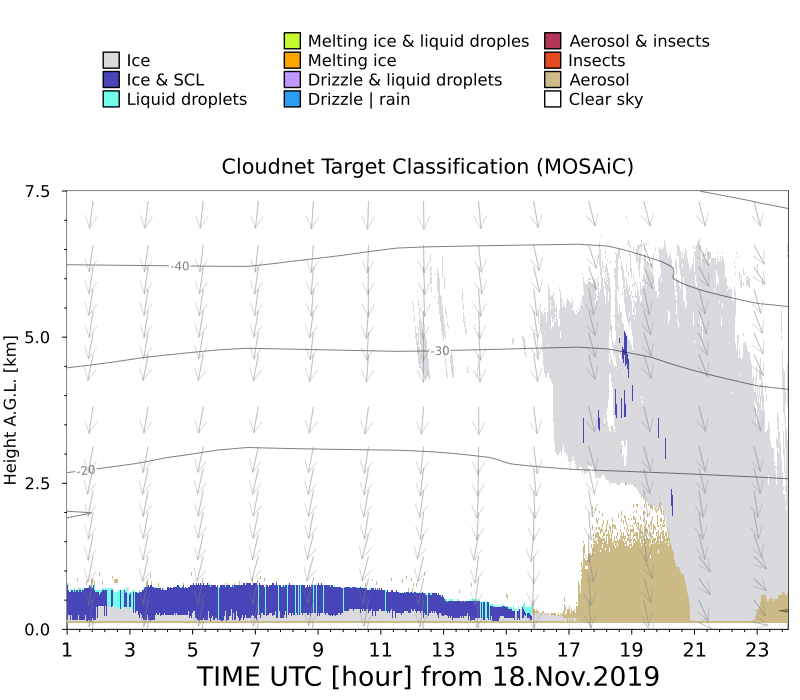
\includegraphics[width=.6\linewidth]{cloudnet_classific_20191118.png}\\
			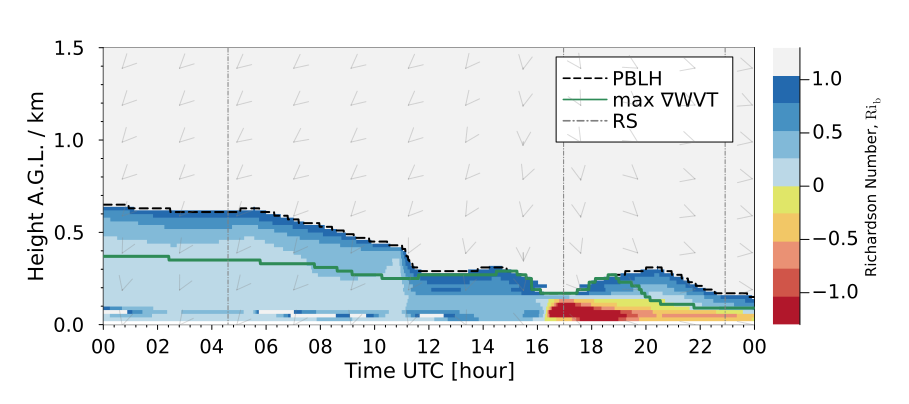
\includegraphics[width=.7\linewidth]{bulk_richardson_number_20191118.png}\\
			\captionof{figure}{Top: Cloudnet classification output from the measurements in Fig.~\ref{fig:measurements}. Bottom: bulk Richardson number for the lowest 1.5~km, with critical $Ri_b$=1 as threshold for PBLH.}
			\label{fig:classification}
		\end{center}
	\end{minipage}
	\end{tabular}
	%\multicolumn{2}{l}{\vspace{+5em}
	
	\colouredcircle {\larger Additional to the Cloudnet target classification (Fig.~\ref{fig:classification}, top), cloud bottom and top heights are estimated for up to four cloud layers.}.To estimating cloud bottom the Cloudnet pixels with liquid droplets or super-cooled liquid (SCL) are considered, for cloud top the ice pixels are added to that (Fig.~\ref{fig:closeup}).\\
\begin{tabular}{ccc}
	%\textbf{\Large COUPLED}	& \textbf{\Large DECOUPLED} \\
	\begin{minipage}{0.3\linewidth}
		\begin{center}
			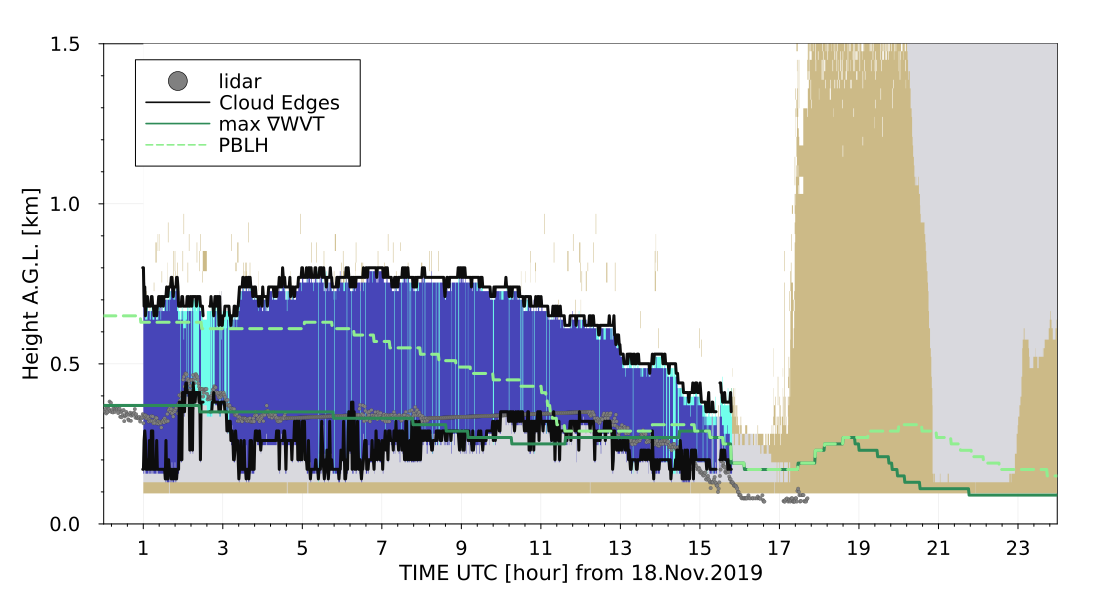
\includegraphics[width=.9\linewidth]{PBLH_zoom_cloudnet_classific_20191118}	
			\captionsetup{width=0.8\linewidth}
			\captionof{figure}{Close-up of Fig.~\ref{fig:classification} (top) for the lowest 1.5~km showing results for the PBLH (dashed-light-green), max~$\nabla WVT$ (green), and estimated cloud bottom and top heights (black lines), the dotted-grey in the cloud base as detected by the ceilometer.}
			\label{fig:closeup}
		\end{center}
	\end{minipage}
	&
	\begin{minipage}{0.32\linewidth}
		Using Cloudnet liquid and ice water content retrievals (lwc \& iwc, respectively), the total path integrated is calculated from cloud bottom to top heights for individual cloud layers: 
		\begin{equation}
			\vspace*{0em}
			\textrm{WP}_{layer}\,=\,\int_{bot}^{top}q_{wc}(z)dz
			\label{eq:lwp}
		\end{equation}
	with $q_{wc}$ being lwc or iwc for liquid or ice water path (LWP, IWP) in Fig.~\ref{fig:lwp}.
		\begin{center}             
			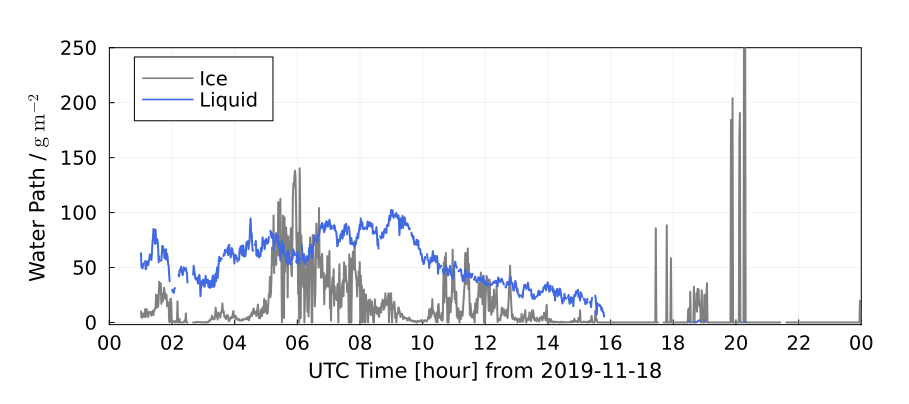
\includegraphics[width=.9\linewidth]{IWP_LWP_timeseries_20191118}
			\captionof{figure}{Liquid and Ice water path for the lowest cloud layer detected in Fig.~\ref{fig:closeup} using Eq.~\ref{eq:lwp}.}
			\label{fig:lwp}
		\end{center}
	\end{minipage}
	&
	\begin{minipage}{0.32\linewidth}
		The wind direction at max~$\nabla WVT$ provides the relevant information to link sea ice LF to the cloud observation above \polarstern. LF is considered form a region determined by the wind direction with center at \polarstern to 50~km radius (grey lines in Fig.~\ref{fig:lf_sic}, right).
		\begin{center}
			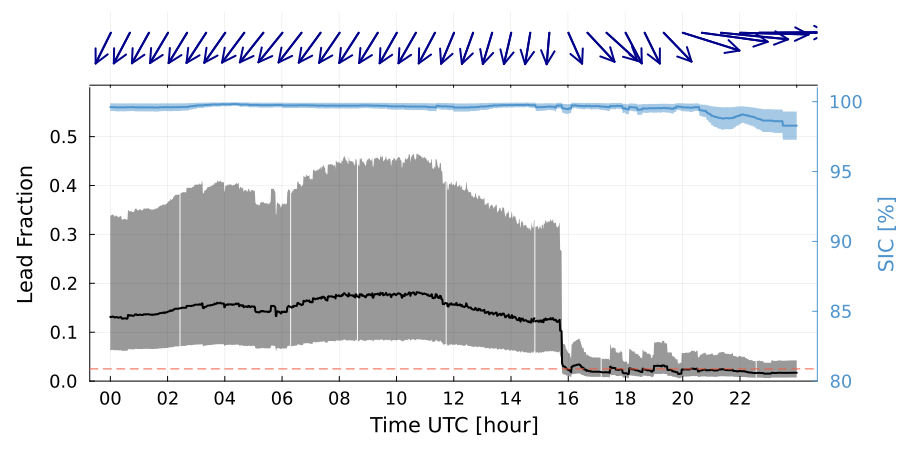
\includegraphics[width=.92\linewidth]{leadfraction_sic_wvtdir_18112019}	
			%\captionsetup{width=0.8\linewidth}
			\captionof{figure}{LF extracted from Fig.~\ref{fig:lf_sic} (right) based on 1-minute wind direction at the max $\nabla WVT$. For reference the the wind vectors at max $\nabla WVT$ (top panel) and SIC for the same region is also shown on light-blue (right axis).}
			\label{fig:wdirwvt}
		\end{center}
		
	\end{minipage}
\end{tabular}
	
	\colouredcircle {\larger From Fig.~\ref{fig:wdirwvt} the 1-minute LF statistics can be related to the corresponding micro- and macrophysical properties of clouds derived from Cloudnet. In order to reduce variability the following results are averaged in 15~minutes intervals i.e. every point represents $\approx$ 15 observations and bars are their variance within it.}\\
\begin{minipage}{0.99\linewidth}
	%\setcaptiontype{figure}
	\centering
	%\subfloat
	[a]{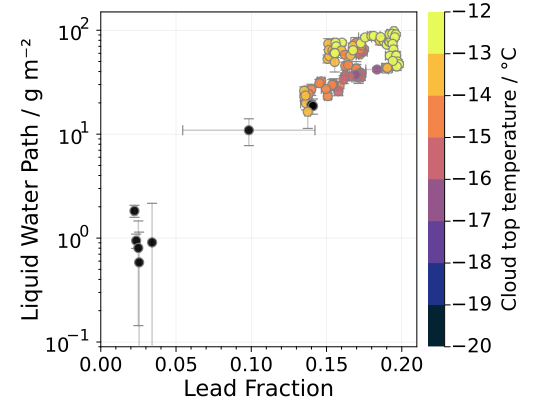
\includegraphics[width=.28\linewidth]{LWP_LF_20191118}}\hfill
	%\subfloat
	[b]{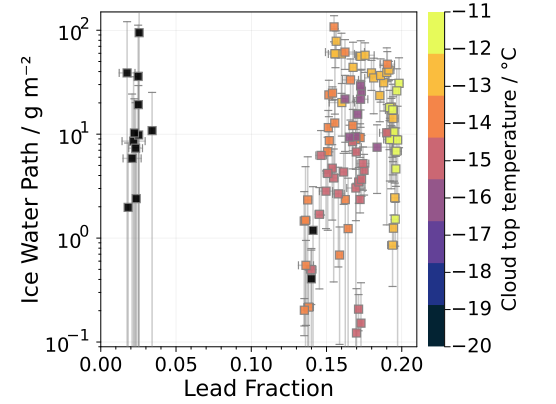
\includegraphics[width=.28\linewidth]{IWP_LF_20191118}}\hfill
	%\subfloat
	[c]{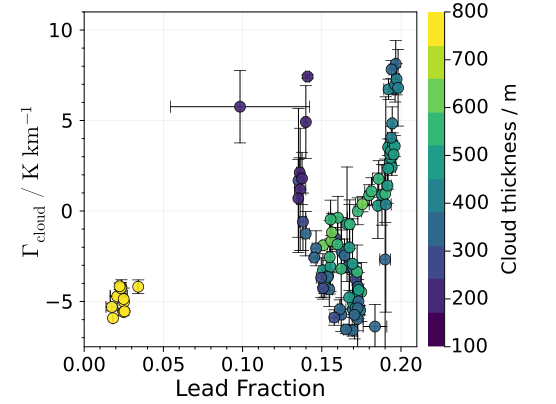
\includegraphics[width=.28\linewidth]{LPRcloud_LF_20191118.png}}
	\captionsetup{width=0.8\linewidth}
	\captionof{figure}{[a]~mean single cloud layer LWP vs. LF (black-line in Fig.~\ref{fig:wdirwvt}) with colour-coded cloud top temperature. [b]~Same but for IWP of same cloud layer. [c]~$\Gamma_{\rm cloud}$ as defined in Eq. vs. LF with colour-coded cloud thickness.}
	\label{fig:scatterWPLF}
\end{minipage}\\

From Fig.~\ref{fig:scatterWPLF} [a] a clear relationship of LWP and LF can be seen, the larger the LF the higher LWP, and the warmer the cloud top temperature too. For IWP (Fig.~\ref{fig:scatterWPLF} [b]) there is no relationship, with a wide range of IWP values the observed LF. The only clear feature is the clustering of points with coupled cases being gathered towards larger LF. Shown in Fig.~\ref{fig:scatterWPLF} [c] is the gradient of cloud temperature as defined by $\Gamma_{\rm cloud}=\frac{\Delta T}{\Delta H}$ (with $\Delta T=T_{top}-T_{bot}$ and $\Delta H=CTH-CBH$) vs. LF with colour-coded cloud thickness. The most negative $\Gamma_{\rm cloud}$ are closer to a moist adiabatic lapse-rates, whereas positive values indicates inversion at cloud top, however this is not consistent neither with increasing LF nor thickness since for coupled cases there are positive and negative $\Gamma_{\rm cloud}$ which is an indicator of other factors affecting it.
   
%\parbox[l]{0.8\linewidth}{   \vspace{-.5em}
%	{Some text here....}    
%}
}

%%%%%%%%%%%%%%%%%%%%%%%%%%%%%%%%%%%%%%%%%%%%%%%%%%%%%%%%%%%%%%%%%%%%%%%%%%%%%%
\headerbox{4.- Conclusions}{name=conclutions,column=0,span=2,below=methods}{
  %%%%%%%%%%%%%%%%%%%%%%%%%%%%%%%%%%%%%%%%%%%%%%%%%%%%%%%%%%%%%%%%%%%%%%%%%%%%%%
{\small
\begin{itemize}
		\item By coupling cloud observations with LF downwind with water vapour trasport as conveying mechanishm for the coupling, seems to be plausible,
		\item A positive relationship LWP and LF has been found, the same is not found for IWP or cloud temperature gradient,
		\item Larger LF are acompained by warmer cloud top, indicating a higher moisture content for those cases,
		\item It is confirmed that uncoupled clouds are mostly high level clouds~\ref{bib:garfias2021},
		\item SAR based LF at 700~, spatial resolution are crutial, the same results cannot be reproduce by usind passive SIC retrievals at 1~km resolution,
		%Results are consistent with previous findings regarding the effect of low sea ice concentration (e.g., due to the presence of leads or polynyas) on cloud micro- and macro-physical properties~[\ref{bib:garfias2021}].
		%\item Cloud properties like liquid and ice water path (LWP and IWP), cloud base height, and cloud geometrical thickness are also variables strongly influencing the surface radiation budget.
		%\item Our results depict a warming cloud effect on the surface is clearly enhanced by atmospheric thermodynamic and dynamic conditions which yiel coupling with the sea ice situation downwind.
\end{itemize}

Statistics based on this methodology are being prepared for the whole \mosaic wintertime expedition in order enrich the results based on this case study.
}
% \sc (this make cool big font)!
}

%%%%%%%%%%%%%%%%%%%%%%%%%%%%%%%%%%%%%%%%%%%%%%%%%%%%%%%%%%%%%%%%%%%%%%%%%%%%%%
\headerbox{5.- References }{name=references,column=0, span=3, below=conclutions}{
%%%%%%%%%%%%%%%%%%%%%%%%%%%%%%%%%%%%%%%%%%%%%%%%%%%%%%%%%%%%%%%%%%%%%%%%%%%%%%
%\colouredcircle \hspace{2em}
\hspace{-2.4em}
\begin{minipage}{0.99\linewidth}
{\smaller
	\begin{enumerate}
		\setlength\itemsep{0.08em}
		\item \label{bib:Shupe2022}Shupe, M. et al. "Overview of the \mosaic
		expedition~{Atmosphere}, Elementa: Science of the Anthropocene, doi:10.1525/elementa.2021.00060, (2022).
		\item \label{bib:Ebell2022}Ebell, K. et al. "Temperature and humidity profiles, integrated water vapour and liquid water path derived from the HATPRO microwave radiometer onboard the Polarstern during the MOSAiC expedition", doi:10.1594/PANGAEA.941389, (2022).
		\item \label{bib:Tukiainen2020}Tukiainen, S. et al. "CloudnetPy: A Python package for processing cloud remote sensing data", JOSS, doi:10.21105/joss.02123, (2020).
		\item \label{bib:vonAlbedyll2021}von~Albedyll, L. et al. "Linking sea ice deformation to ice thickness redistribution using high-resolution satellite and airborne observations", The Cryosphere, doi:10.5194/tc-15-2167-2021, (2021).
		\item \label{bib:Ludwig2021}Ludwig, V., Spreen, G. et al. "Evaluation of a {New} {Merged} {Sea}-{Ice} {Concentration} {Dataset} at 1 ~m {Resolution} from {Thermal} {Infrared} and {Passive} {Microwave} {Satellite} {Data} in the {Arctic}", Remote Sensing, doi:10.3390/rs12193183, (2020).
		\item \label{bib:garfias2021}Saavedra~Garfias, P., Kalesse-Los, H. et al. "Climatology of clouds containing supercooled liquid in the Western and Central Arctic". American Geophysical Union (2021), ESSOAR. DOI10.1002/essoar.10509918.1
		\item \label{bib:jannos2022}Michaelis J, Lüpkes C. "The Impact of Lead Patterns on Mean Profiles of Wind, Temperature, and Turbulent Fluxes in the Atmospheric Boundary Layer over Sea Ice". Atmosphere. (2022) https://doi.org/10.3390/atmos13010148 
	\end{enumerate}
}	
\vspace{-0.6em}
\end{minipage}
	%\end{tabular}
	%\vspace{0.5em}
}
%%%%%%%%%%%%%%%%%%%%%%%%%%%%%%%%%%%%%%%%%%%%%%%%%%%%%%%%%%%%%%%%%%%%%%%%%%%%%%
\headerbox{Acknowledges}{name=acknown,column=2, span=1, below=methods}{
	%%%%%%%%%%%%%%%%%%%%%%%%%%%%%%%%%%%%%%%%%%%%%%%%%%%%%%%%%%%%%%%%%%%%%%%%%%%%%%
	{\smaller This work is supported by the DFG funded Transregio-project TR-172 "Arctic Amplification $(AC)^3$". Authors thank to DOE ARM program for providing \mosaic data as well as the whole \mosaic community. SIC product is obtained from the University of Bremen under supported by Dr. Gunnar Spreen. Cloud classification performed with open-source \emph{Cloudnetpy} by ACTRIS and FMI.
	}\\{\large \textbf Gedruckt im Universitätsrechenzentrum Leipzig}
}
%\headerbox{[*] Contact}{name=contact, column=2, below=results}{
%{\Large \color{white}{Email:	pablo.saavedra@uni-leipzig.de}}\\
%\hspace{3em}%\includegraphics[scale=0.04]{github_pablosaa.png}\hspace{3em}
%\includegraphics[scale=0.16]{twitter_DunkleWolke.png}
%}

\end{poster}

\end{document}

%%%%%%%%%%%%%%%%%%%%%%%%%%%%%%%%%%%%%%%%%%%%%%%%%%%%%%%%%%%%%%%%%%%%%%%%%%%%%%%
